\documentclass[tikz,border=0pt]{standalone}
\usepackage{amsmath, amssymb}
\usetikzlibrary{matrix, positioning, fit, backgrounds, calc}

\usepackage{helvet}
\usepackage{avant}
\renewcommand*\familydefault{\sfdefault}
\usepackage{textcomp}

\usepackage{fontspec}
\setmainfont{TeX Gyre Termes}
\setsansfont[
Path = fonts/,
UprightFont = *Medium.ttf,
BoldFont    = *Bold.ttf,
AutoFakeSlant = 0.2
]{GmarketSansTTF}
\begin{document}
	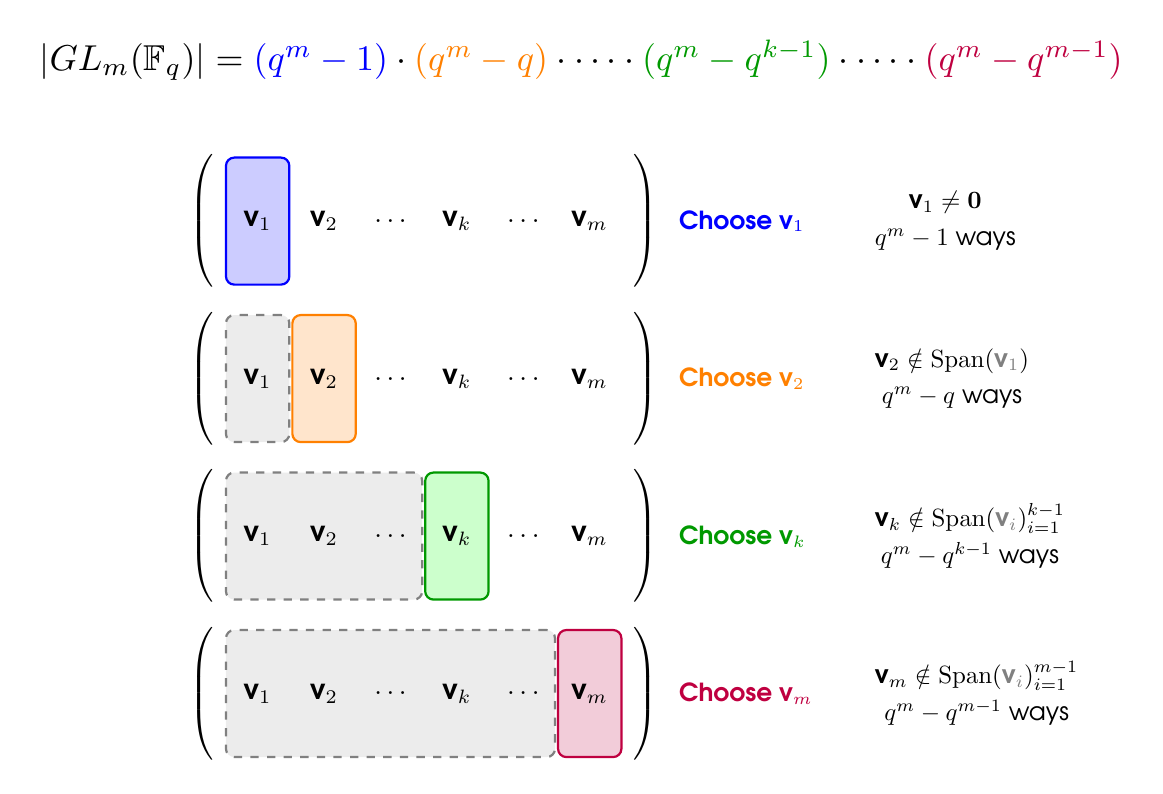
\begin{tikzpicture}[
		font=\sffamily,
		% Style for block-column matrices
		mtx/.style={
			matrix of math nodes,
			left delimiter=(, right delimiter=),
			% Make nodes tall to accurately represent full column vectors
			nodes={minimum width=2.2em, minimum height=4.5em, inner sep=2pt, anchor=center},
			column sep=2pt, row sep=0pt,
			ampersand replacement=\&
		},
		% Highlighting styles for active columns
		hl-v1/.style={fill=blue!20, draw=blue, thick, rounded corners=3pt, inner sep=.25pt},
		hl-v2/.style={fill=orange!20, draw=orange, thick, rounded corners=3pt, inner sep=.25pt},
		hl-vk/.style={fill=green!20, draw=green!60!black, thick, rounded corners=3pt, inner sep=.25pt},
		hl-vm/.style={fill=purple!20, draw=purple, thick, rounded corners=3pt, inner sep=.25pt},
		% Style for the forbidden "Span" subspace
		hl-span/.style={fill=gray!15, draw=gray, dashed, thick, rounded corners=3pt, inner sep=.25pt},
		% Connector styles
		arrow/.style={->, >=latex, thick, shorten >=2pt},
		term label/.style={font=\bfseries\small, align=center}
		]
		
		% ==============================================================================
		% 1. MAIN TITLE & EQUATION
		% ==============================================================================
%		\node[font=\sffamily\bfseries\LARGE, color=darkgray, align=center] (title) at (0, 7) {Structural Generalization: $m \times m$ Matrix over $\mathbb{F}_q$};
		
		\node[scale=1.3] (eq) at (0, 0) {
			$|GL_m(\mathbb{F}_q)| = 
			\textcolor{blue}{(q^m - 1)} \cdot 
			\textcolor{orange}{(q^m - q)} \cdot 
			\dots \cdot 
			\textcolor{green!60!black}{(q^m - q^{k-1})} \cdot 
			\dots \cdot 
			\textcolor{purple}{(q^m - q^{m-1})}$
		};
		
		% Reference node for vertical spacing
		\node[below=1.5cm of eq] (center_node) {};
		
		% ==============================================================================
		% 2. BRANCH 1: First Column (v1)
		% ==============================================================================
		\matrix[mtx] (M1) at ($(center_node)+(-2,0)$) {
			\textbf{v}_1 \& \textbf{v}_2 \& \dots \& \textbf{v}_k \& \dots \& \textbf{v}_m \\
		};
		\begin{scope}[on background layer]
			\node[hl-v1, fit=(M1-1-1)] {};
		\end{scope}
		\node[right=0.5cm of M1, term label, text=blue] {Choose $\textbf{v}_1$};
		\node[right=3cm of M1, scale=0.9, align=center] {
			$\textbf{v}_1 \neq \mathbf{0}$ \\[1mm]
%			$\mathrm{dim}(\emptyset) = 0 \implies q^{0}$ elements  \\[1mm]
			\textbf{$q^m - 1$} ways
		};
		
		% ==============================================================================
		% 3. BRANCH 2: Second Column (v2)
		% ==============================================================================
		\matrix[mtx] (M2) at ($(center_node)+(-2, -2)$) {
			\textbf{v}_1 \& \textbf{v}_2 \& \dots \& \textbf{v}_k \& \dots \& \textbf{v}_m \\
		};
		\begin{scope}[on background layer]
			\node[hl-span, fit=(M2-1-1)] {};
			\node[hl-v2, fit=(M2-1-2)] {};
		\end{scope}
		\node[right=0.5cm of M2, term label, text=orange] {Choose $\textbf{v}_2$};
		\node[right=3cm of M2, scale=0.9, align=center] {
			$\textbf{v}_2 \notin \mathrm{Span}(\textcolor{gray}{\textbf{v}_1})$ \\[1mm]
%			$\mathrm{dim} = 1 \implies q^1$ elements \\[1mm]
			\textbf{$q^m - q$} ways
		};
		
		% ==============================================================================
		% 4. BRANCH k: General k-th Column (vk)
		% ==============================================================================
		\matrix[mtx] (Mk) at ($(center_node)+(-2, -4)$) {
			\textbf{v}_1 \& \textbf{v}_2 \& \dots \& \textbf{v}_k \& \dots \& \textbf{v}_m \\
		};
		\begin{scope}[on background layer]
			\node[hl-span, fit=(Mk-1-1)(Mk-1-3)] {};
			\node[hl-vk, fit=(Mk-1-4)] {};
		\end{scope}
		\node[right=0.5cm of Mk, term label, text=green!60!black] {Choose $\textbf{v}_k$};
		\node[right=3cm of Mk, scale=0.9, align=center] {
			$\textbf{v}_k \notin \mathrm{Span}(\textcolor{gray}{\textbf{v}_i})_{i=1}^{k-1}$ \\[1mm]
%			$\mathrm{dim} = k-1 \implies q^{k-1}$ elements \\[1mm]
			\textbf{$q^m - q^{k-1}$} ways
		};
		
		% ==============================================================================
		% 5. BRANCH m: Final Column (vm)
		% ==============================================================================
		\matrix[mtx] (Mm) at ($(center_node)+(-2, -6)$) {
			\textbf{v}_1 \& \textbf{v}_2 \& \dots \& \textbf{v}_k \& \dots \& \textbf{v}_m \\
		};
		\begin{scope}[on background layer]
			\node[hl-span, fit=(Mm-1-1)(Mm-1-5)] {};
			\node[hl-vm, fit=(Mm-1-6)] {};
		\end{scope}
		\node[right=0.5cm of Mm, term label, text=purple] {Choose $\textbf{v}_m$};
		\node[right=3cm of Mm, scale=0.9, align=center] {
			$\textbf{v}_m \notin \mathrm{Span}(\textcolor{gray}{\textbf{v}_i})_{i=1}^{m-1}$ \\[1mm]
%			$\mathrm{dim} = m-1 \implies q^{m-1}$ elements \\[1mm]
			\textbf{$q^m - q^{m-1}$} ways
		};
		
		% ==============================================================================
		% 6. ARROWS AND MULTIPLICATION SIGNS
		% ==============================================================================
		
		% Arrows linking equation to matrices
%		\draw[arrow, blue] ($(eq.south)+(-4.5,0)$) to[out=270, in=90] (M1.north);
%		\draw[arrow, orange] ($(eq.south)+(-2.5,0)$) to[out=270, in=90] (M2.north);
%		\draw[arrow, green!60!black] ($(eq.south)+(1.8,0)$) to[out=270, in=90] (Mk.north);
%		\draw[arrow, purple] ($(eq.south)+(5.2,0)$) to[out=270, in=90] (Mm.north);
%		
%		% Multiplication dots between the matrix visual blocks
%		\node[scale=2, text=gray] at ($(M1)!0.5!(M2)+(0,-1.3)$) {$\times$};
%		\node[scale=2, text=gray] at ($(M2)!0.5!(Mk)+(0,-1.3)$) {$\dots$};
%		\node[scale=2, text=gray] at ($(Mk)!0.5!(Mm)+(0,-1.3)$) {$\dots$};
	\end{tikzpicture}
\end{document}